104. \begin{figure}[ht!]
\center{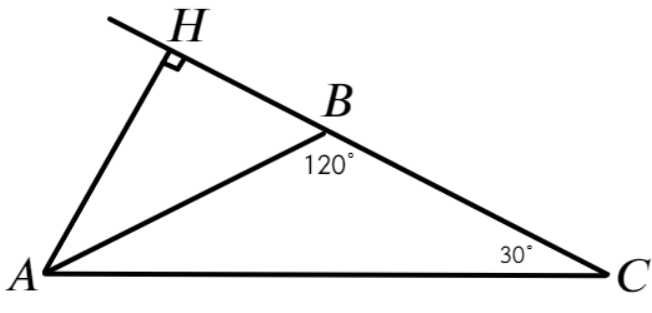
\includegraphics[scale=0.35]{g8-103.png}}
\end{figure}\\
Найдём $\angle C=\angle A=(180^\circ-120^\circ):2=30^\circ.$ Тогда в прямоугольном треугольнике $AHC$ катет $AH$ лежит напротив угла в $30^\circ$ и
$AH=\cfrac{1}{2}AC=\cfrac{1}{2}\cdot30=15$см.\\
